Die Musterl�sung wurde mit den in Abb. \ref{fig:A1_01} eingestellten Paramteren erstellt
\begin{figure}[ht]
\centering 
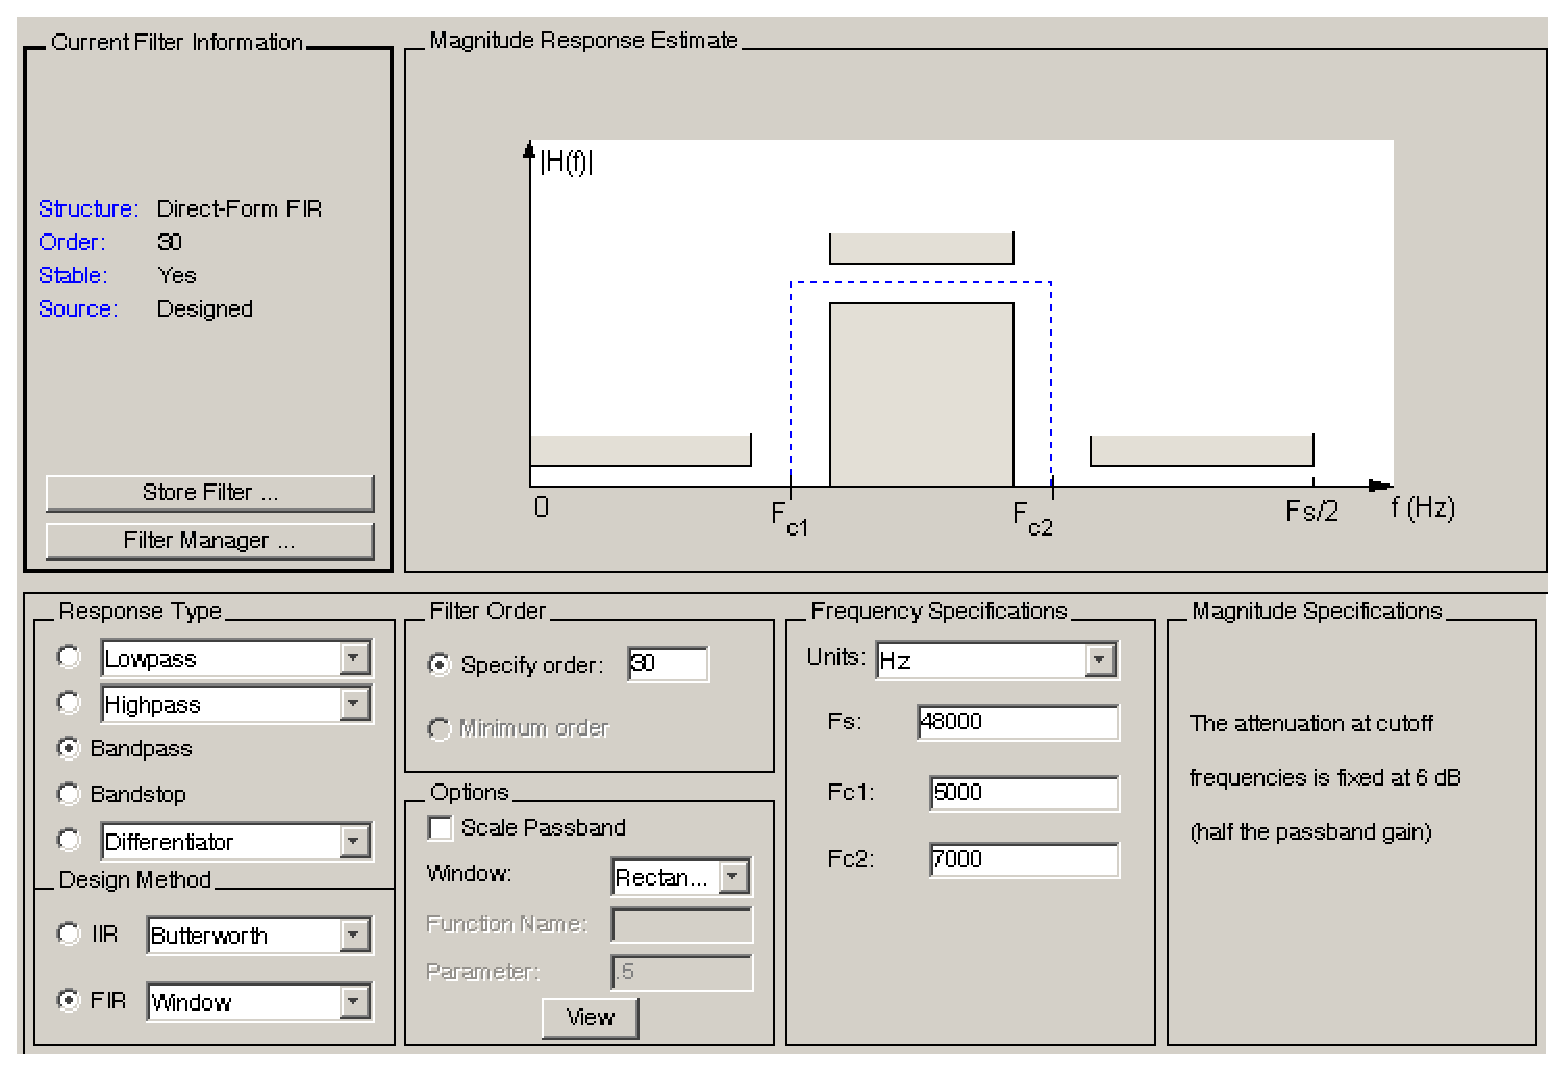
\includegraphics[width=4cm]{bilder/empf�nger/filterdesign/BPWinPar}
\caption{Eingestellte Parameter}
\label{fig:A1_01}
\end{figure}

Die Abb. \ref{fig:A1_02} und \ref{fig:A1_03} Stellen das verwendete Rechteck-Fenster und den 						resultierenden 
Ampitudenverlauf des Filters dar.
\begin{figure}[ht]
\centering 
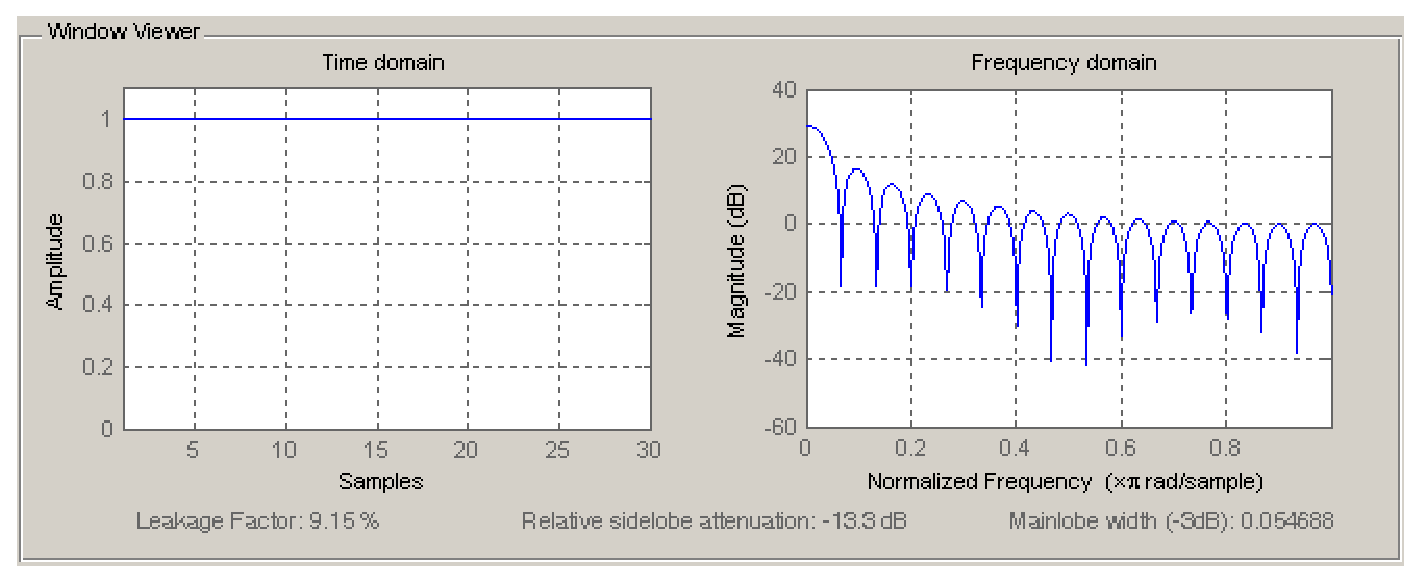
\includegraphics[width=4cm]{bilder/empf�nger/filterdesign/Rechteckfenster}
\caption{Rechteckfenster}
\label{fig:A1_02}
\end{figure}
		
\begin{figure}[ht]
\centering 
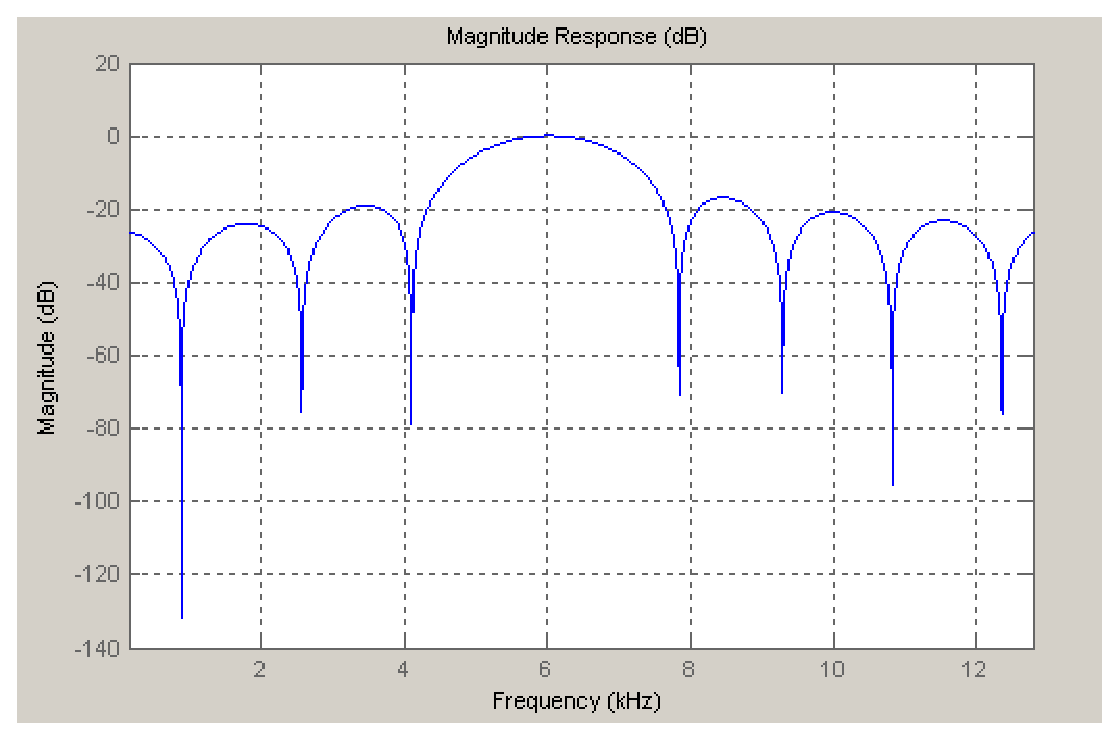
\includegraphics[width=4cm]{bilder/empf�nger/filterdesign/BPWinRect}
\caption{Frequenzgang mit Rechteckfenster}
\label{fig:A1_03}
\end{figure}
		
Jetzt das Ganze nochmal mit einem Hanning-Fenster (Abb. \ref{fig:A1_04} \ref{fig:A1_05}
\begin{figure}[ht]
\centering 
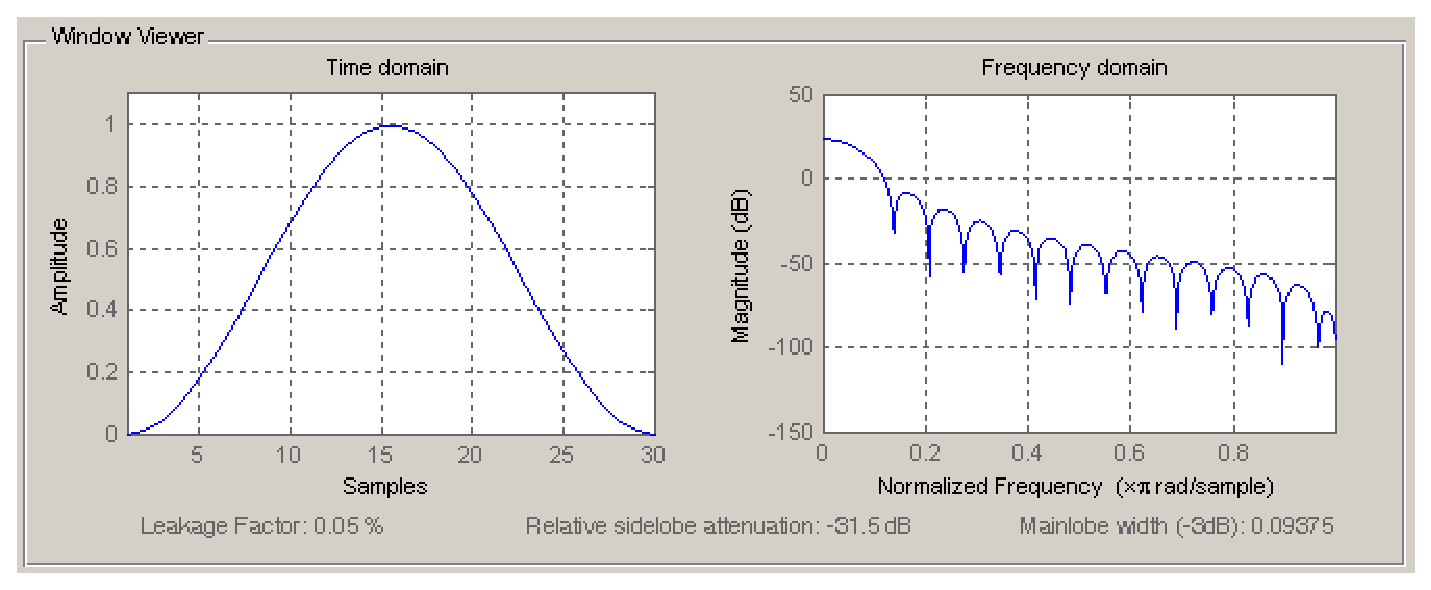
\includegraphics[width=4cm]{bilder/empf�nger/filterdesign/Hanning}
\caption{Hanningfenster}
\label{fig:A1_04}
\end{figure}
		
\begin{figure}[ht]
\centering 
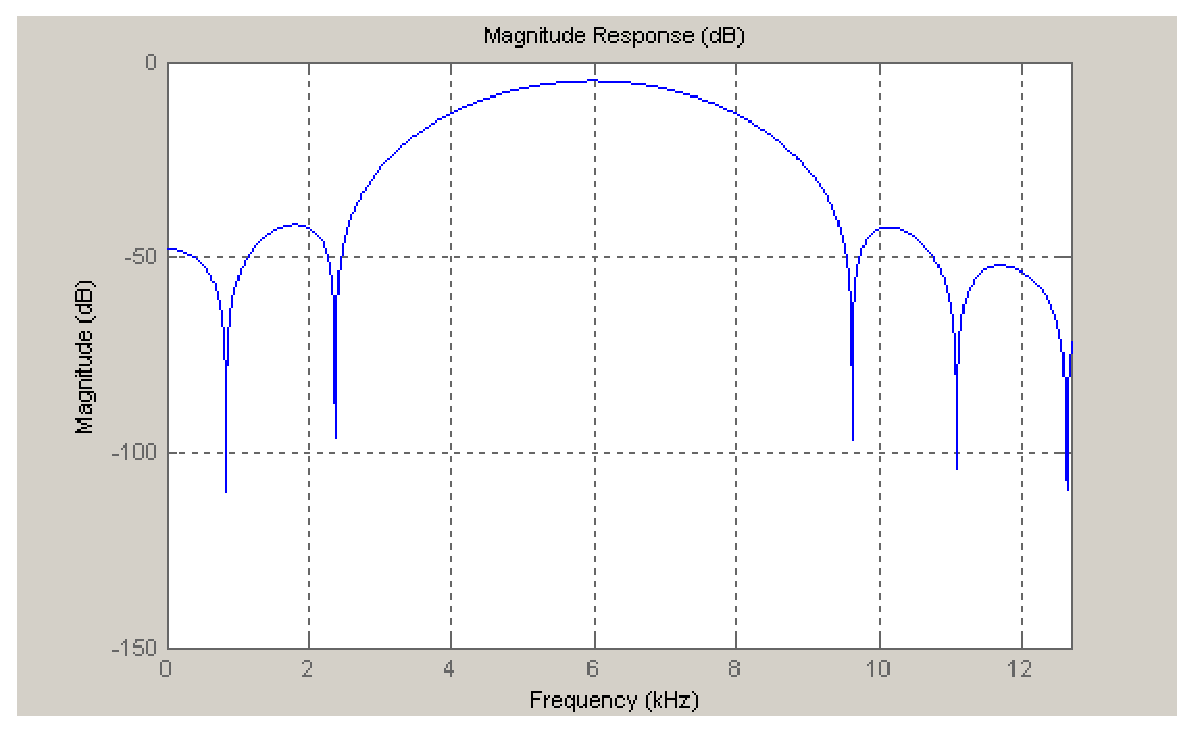
\includegraphics[width=4cm]{bilder/empf�nger/filterdesign/BPWinHann}
\caption{Frequenzgang mit Hanningfenster}
\label{fig:A1_05}
\end{figure}

Zum Abschluss noch mit dem Kaiserfenster (Parameter Beta: 1.8; Abb. \ref{fig:A1_06} und 								\ref{fig:A1_07})
\begin{figure}[ht]
\centering 
\includegraphics[width=4cm]{bilder/empf�nger/filterdesign/Kaiser}
\caption{Kaiserfenster, Beta: 1.8}
\label{fig:A1_06}
\end{figure}
		
\begin{figure}[ht]
\centering 
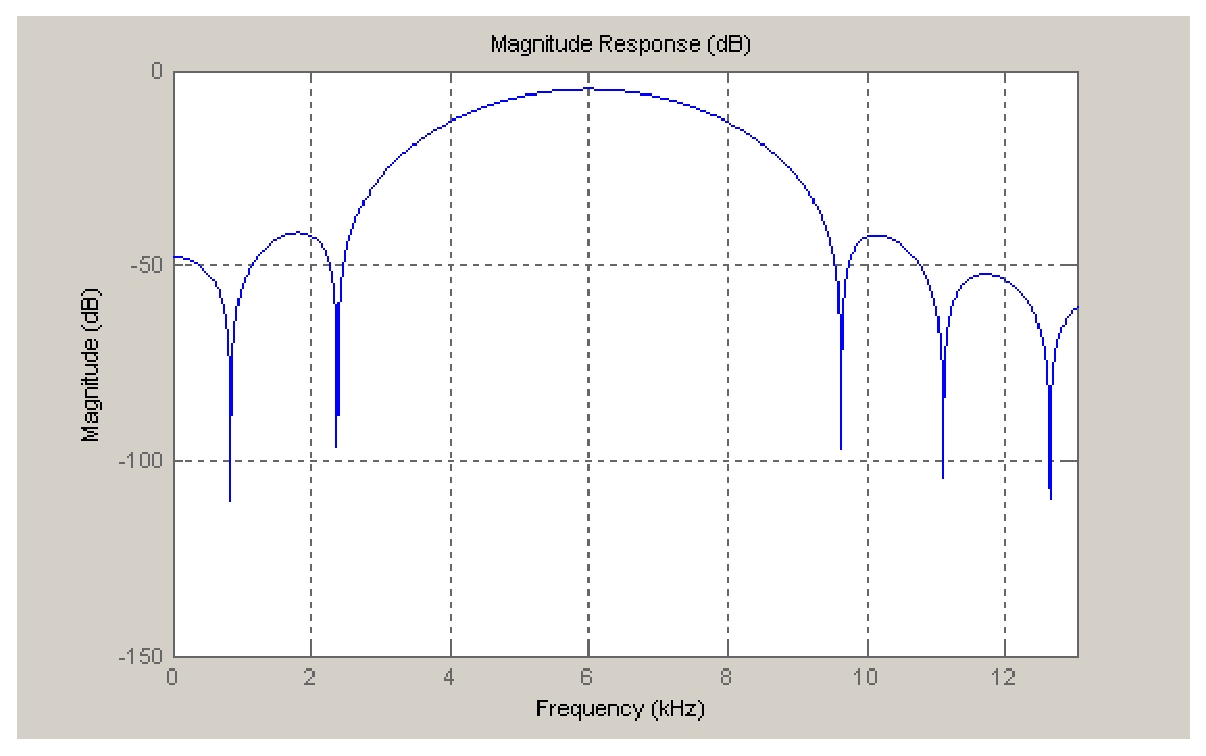
\includegraphics[width=4cm]{bilder/empf�nger/filterdesign/BPWinKaiser}
\caption{Frequenzgang mit Kaiserfenster}
\label{fig:A1_07}
\end{figure}		